%!TEX root = ../../book_ML.tex
\chapter{Cơ sở lý thuyết}
\label{cha: chap2}
% \index{principal component analysis}
% \index{PCA -- \textit{xem} principle component analysis}
% \index{PCA}

% \index{phân tích thành phần chính -- principle component analysis}
% \index{principle component analysis -- phân tích thành phần chính}
% \index{PCA}
\section{Tổng quan về nhận diện khuôn mặt}

Nhận diện khuôn mặt (Face recogintion) đang được ứng dụng trong nhiều lĩnh vực.
Hệ thống nhận dạng khuôn mặt là một ứng dụng cho phép máy tính tự động xác định
hoặc nhận dạng một người nào đó từ một bức hình ảnh kỹ thuật số hoặc một khung
hình.

Nhận diện khuôn mặt là một bài toán phức tạp, đòi hỏi cần phải xử lý một
loạt các vấn đề.

Mỗi khuôn mặt đều có nhưng điểm mốc, những phần lồi lõm, hình dáng của các
bộ phận trên khuôn mặt như mắt, mũi, miệng,... Các hệ thống nhận diện định
nghĩa những điểm này là những điểm nút, và mỗi khuôn mặt có khoảng 80 nút như thế.

Ngày nay các mô hình học sâu đã phát triển một cách vượt trội, việc trích rút các đặc trưng của một
khuôn mặt ngày một đơn giản và trở lên vô cùng chính xác. Mặc dù chúng ta không thể biết các đặc trưng đấy
là những đặc trưng gì bởi cơ chế tự động học của các mô hình học sâu rất phức tạp. Nhưng chúng ta vẫn có thể
kiểm tra độ chính xác bằng cách đưa những đặc trưng này vào các mô hình phân loại, xác nhận, ... sau đó
tính toán độ chính xác trên những dữ liệu có được.


\section{Tìm hiểu về OpenCV và ngôn ngữ lập trình Python}

OpenCV (Open Source Computer Vision Library) là một thư viện các chức năng lập
trình chủ yếu nhắm vào tầm nhìn máy tính thời gian thực. OpenCV hỗ trợ nhiều ngôn
ngữ lập trình như C++, Python, Java,… và có sẵn trên các nền tảng khác nhau bao
gồm Windows, Linux, Mac OS, Android và iOS. Các giao diện cho các hoạt động
GPU tốc độ cao dựa trên CUDA và OpenCL cũng đang được phát triển tích cực.

Cấu trúc tổng quan của OpenCV bao gồm 5 phần chính. 4 trong 5 phần đó được chỉ ra
trong hình vẽ dưới.

\begin{figure}
    \begin{subfigure}{0.7\textwidth}
        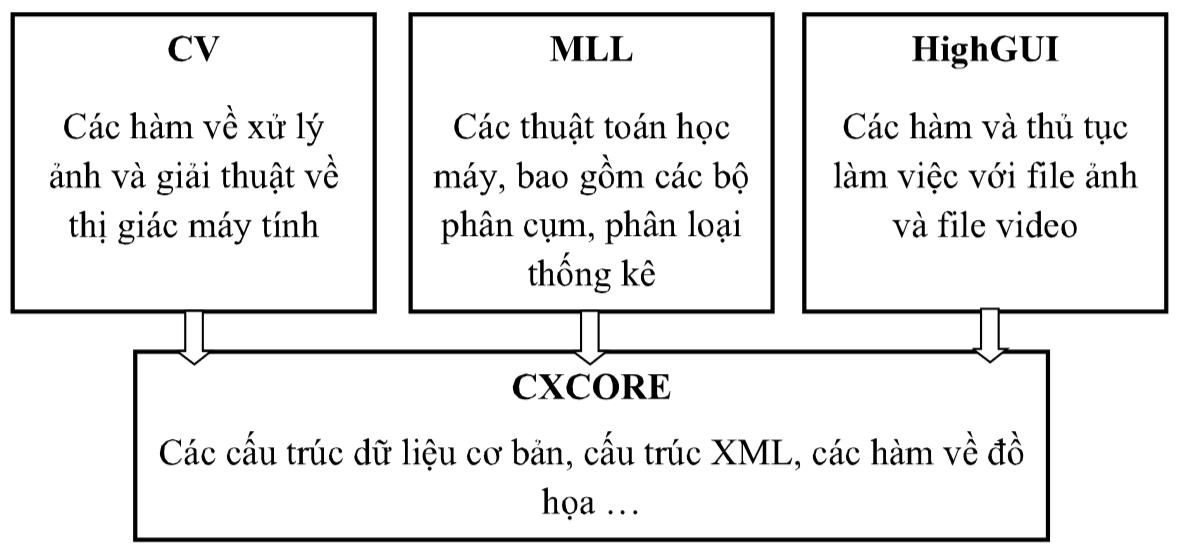
\includegraphics[width=0.99\linewidth]{Chapters/items/chap2_1.jpg}
        \caption{}
        \label{fig: chap2_1}
    \end{subfigure}
    \caption{Cấu trúc các phần của OpenCV.}
\end{figure}

Phần CV bao gồm các thư viện cơ bản về xử lý ảnh và các giải thuật về xử lý ảnh.
MLL là bộ thư viện về các thuật toán học máy, bao gồm rất nhiều bộ phân cụm và phân
loại thống kê. HighGUI chứa đựng những thủ tục vào ra, các chức năng về lưu trữ cũng
như đọc các file ảnh và video. Phần thứ 4, Cxcore chứa đựng các cấu trúc dữ liệu
cơ bản (ví dụ như cấu trúc XML, các cây dữ liệu …). Phần cuối cùng là CvAux, phần này
bao gồm các thư viện cho việc phát hiện, theo dõi và nhận dạng đối tượng (khuôn mặt, mắt …).

OpenCV - Python là một thư viện các ràng buộc Python được thiết kế để giải quyết các vấn đề
về xử lý ảnh và thị giác máy tính.

Python là ngôn ngữ lập trình có mục đích chung được bắt đầu bởi Guido van Rossum,
nó trở nên rất phổ biến rất nhanh trong thời gian gần đây, chủ yếu vì tính đơn giản
và khả năng đọc mã của nó. Nó cho phép lập trình viên thể hiện ý tưởng trong ít dòng
mã hơn mà không làm giảm khả năng đọc.

So với các ngôn ngữ như C/C++, Python chậm hơn. Điều đó nói rằng, Python có thể dễ dàng
được mở rộng với C/C++, cho phép chúng ta viết mã chuyên sâu tính toán trong C/C++
và tạo các trình bao bọc Python có thể được sử dụng làm mô-đun Python.
Điều này mang lại cho chúng ta hai lợi thế: thứ nhất, mã nhanh như mã C/C++ gốc
(vì đây là mã C++ thực tế hoạt động ở chế độ nền) và thứ hai, mã dễ dàng hơn trong
Python so với C/C++. OpenCV - Python là một trình bao bọc Python để thực hiện OpenCV C++
ban đầu.

OpenCV - Python sử dụng Numpy, một thư viện được tối ưu hóa cao cho các hoạt động số với
cú pháp kiểu MATLAB. Tất cả các cấu trúc mảng OpenCV được chuyển đổi sang và từ các mảng
Numpy. Điều này cũng giúp tích hợp dễ dàng hơn với các thư viện khác sử dụng Numpy
như SciPy và Matplotlib.



\section{Mô hình mạng neural tích chập (CNN - Convolutional neural network)}

Mạng neural tích chập (CNN) là một trong những mô hình học sâu\cite{repec} tiên tiến phổ biến nhất và
có ảnh hưởng nhất với cộng đồng thị giác máy tính (Computer vision). CNN thường được dùng
trong các bài toán nhận dạng ảnh, phân tích ảnh, xử lý ngôn ngữ tự nhiên dưới dạng ảnh các bước sóng.
Và hầu hết đều cho hiệu quả tốt đến rất tốt.

CNN là một kiến trúc mạng neural sinh ra để xử lý các dữ liệu phi cấu trúc dạng ảnh. Có 2 loại lớp
chính trong CNN: lớp tích chập (Convolutional layer) và lớp gộp (Pooling layer)

\begin{figure}
    \begin{subfigure}{1.\textwidth}
        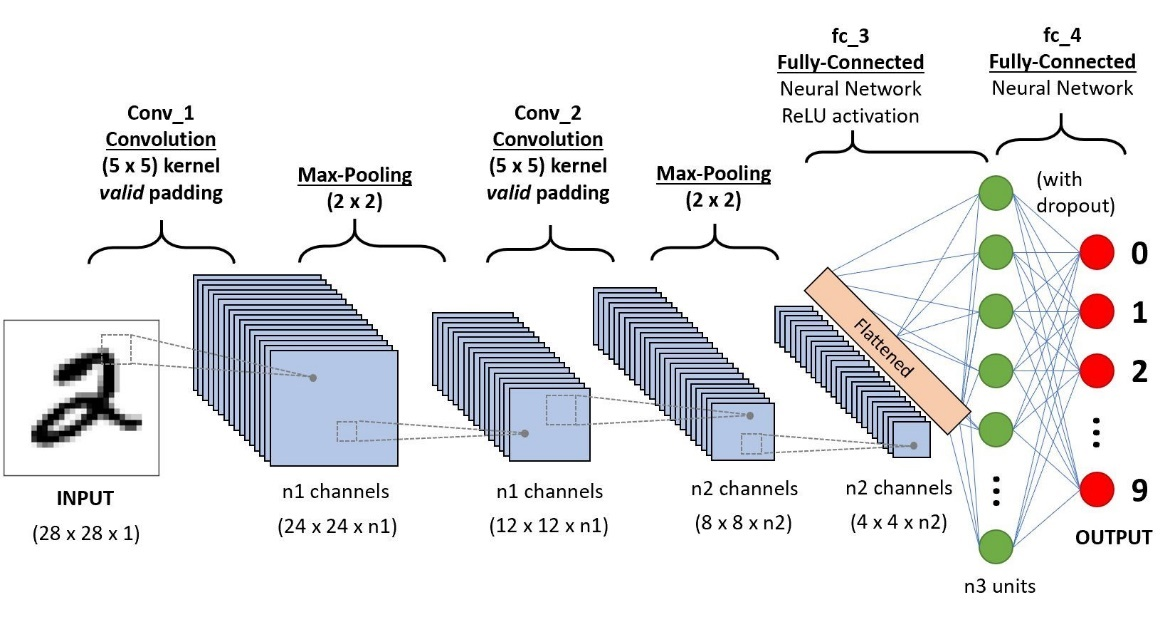
\includegraphics[width=1.\linewidth]{Chapters/items/cnn2_1.jpg}
        \label{fig: chap2_2}
    \end{subfigure}
    \caption{CNN cho bài toán nhận diện chữ số.}
\end{figure}
\subsection{Lớp tích chập}

Lớp tích chập là lớp quan trọng nhất và thường cũng là lớp đầu tiên của của mô hình CNN.
Lớp này có chức năng chính là phát hiện các đặc trưng có tính không gian hiệu quả.
Trong tầng này có 4 đối tượng chính là: ma trận đầu vào, bộ lọc (filters) và trường thụ cảm,
bản đồ đặc trưng (feature map). Lớp tích chập nhận đầu vào là một ma trận 3 chiều và một bộ lọc cần phải học.
Bộ lọc này sẽ trượt qua từng vị trí trên bức ảnh để tính tích chập (convolution)
giữa bộ lọc và phần tương ứng trên bức ảnh. Phần tương ứng này trên bức ảnh gọi là
trường thục cảm (receptive field), tức là vùng mà một neuron có thể nhìn thấy để đưa
ra quyết định, và mà trận cho ra bởi quá trình này được gọi là bản đồ đặc trưng (feature map).

Để hình dung, có thể tưởng tượng, bộ filters giống như các tháp canh trong nhà tù quét
lần lượt qua không gian xung quanh để tìm kiếm tên tù nhân bỏ trốn.
Khi phát hiện tên tù nhân bỏ trốn, thì chuông báo động sẽ reo lên, giống như các bộ lọc
tìm kiếm được đặc trưng nhất định thì tích chập đó sẽ cho giá trị tương ứng.

\begin{enumerate}
    \item Lớp tích chập được coi như xác định đặc trưng
          \begin{itemize}
              \item Lớp tích chập có chức năng chính là phát hiện đặc trưng cụ thể của bức ảnh.
                    Những đặc trưng này bao gồm đặc trưng cơ bản là góc, cạnh, màu sắc, hoặc đặc trưng
                    phức tạp hơn như texture của ảnh. Vì bộ filter quét qua toàn bộ bức ảnh, nên những
                    đặc trưng này có thể nằm ở vị trí bất kì trong bức ảnh, cho dù ảnh bị xoáy trái/phải
                    thì những đặc trưng này vẫn bị phát hiện.
              \item Ở minh họa dưới, có một filter 5x5 dùng để phát hiện góc/cạnh, với filter này
                    chỉ có giá trị một tại các điểm tương ứng một góc cong.
                    \begin{figure}
                        \begin{subfigure}{0.6\textwidth}
                            \begin{center}
                                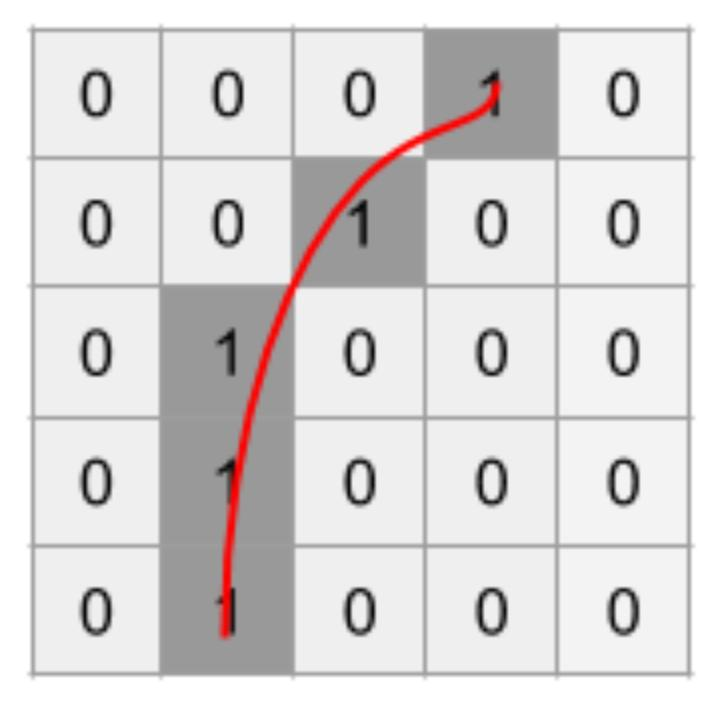
\includegraphics[width=0.6\linewidth]{Chapters/items/chap2_3.jpg}
                            \end{center}
                            \label{fig: chap2_3}
                        \end{subfigure}
                        \caption{Bộ lọc phát hiện cạnh}
                    \end{figure}
              \item Dùng bộ lọc ở trên trược qua ảnh của nhân vật Olaf trong trong bộ phim Frozen.
                    Chúng ta thấy rằng, chỉ ở những vị trí trên bức ảnh có dạng góc như đặc trưng ở
                    bộ lọc thì mới có giá trị lớn trên bản đồ đặc trưng, những vị trí còn lại sẽ cho giá trị
                    thấp hơn. Điều này có nghĩa là, bộ lọc đã phát hiện thành công một dạng góc/cạnh
                    trên dự liệu đầu vào. Tập hơn nhiều bộ lọc sẽ cho phép các bạn phát hiện được
                    nhiều loại đặc trưng khác nhau,và giúp định danh được đối tượng.
                    \begin{figure}
                        \begin{subfigure}{1.\textwidth}
                            \begin{center}
                                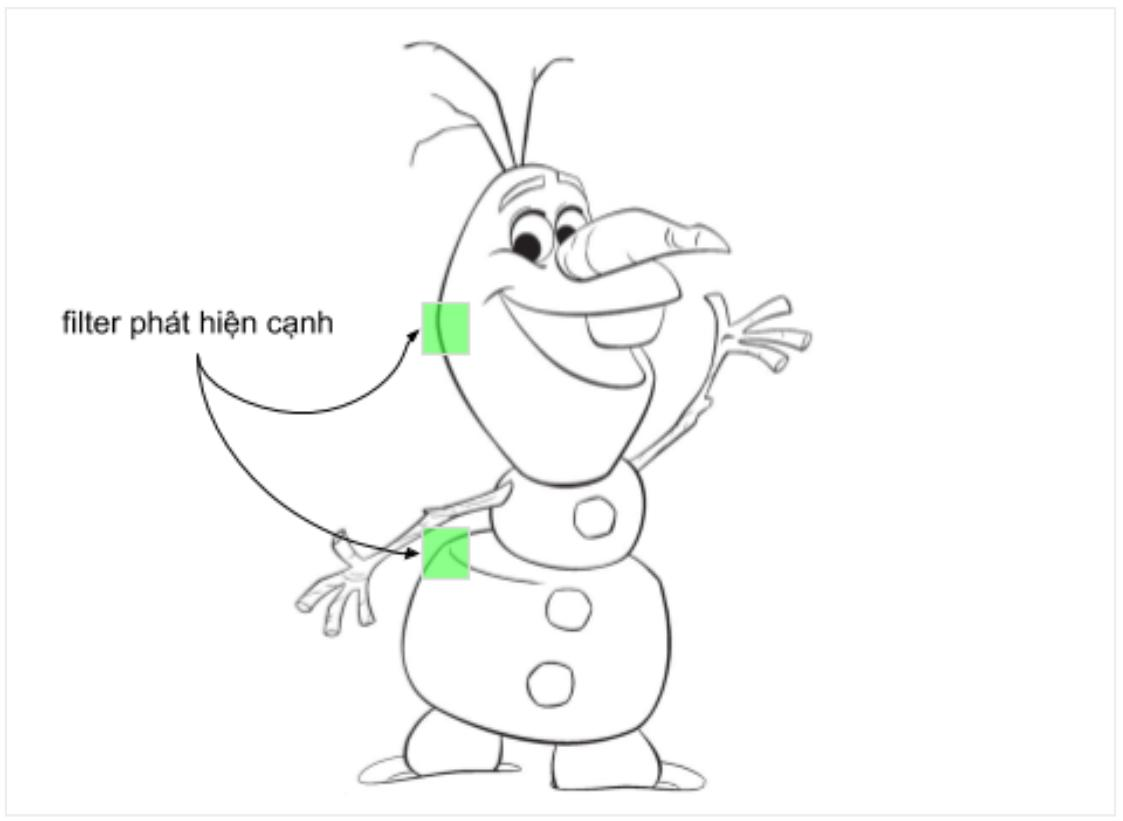
\includegraphics[width=1.\linewidth]{Chapters/items/chap2_4.jpg}
                            \end{center}
                            \label{fig: chap2_4}
                        \end{subfigure}
                        \caption{Bộ lọc phát hiện cạnh}
                    \end{figure}
          \end{itemize}
    \item Các tham số: Kích thước bộ lọc, bước nhảy, lề
          \begin{itemize}
              \item Kích thước bộ lọc là một trong những tham số quan trọng nhất của lớp tích chập.
                    Kích thước này tỉ lệ thuận với số tham số cần học tại mỗi lớp tích chập và
                    là tham số quyết định trường thụ cảm của tầng này. Kích thước phổ biến nhất của bộ lọc
                    là 3x3.
                    \begin{figure}
                        \begin{subfigure}{1.\textwidth}
                            \begin{center}
                                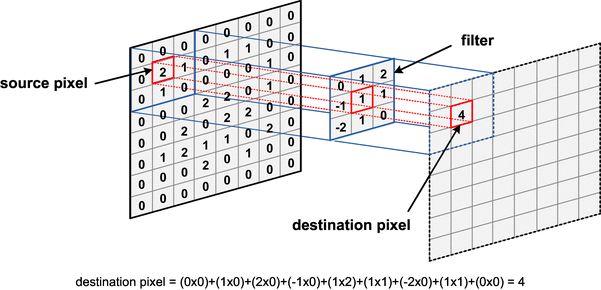
\includegraphics[width=1.\linewidth]{Chapters/items/chap2_5.jpg}
                            \end{center}
                            \label{fig: chap2_5}
                        \end{subfigure}
                        \caption{Cách hoạt động của bộ lọc (filter)}
                    \end{figure}
              \item Kích thước filter nhỏ được ưu tiên lựa chọn thay kích thước lớn vì những lý do sau đây: 
                    \begin{itemize}
                        \item Cho phép nhìn được các vùng nhỏ
                        \item Trích rút được những đặc trưng có tính cục bộ cao
                        \item Phát hiện đặc trưng nhỏ
                        \item Đặc trưng được trích rút sẽ nhiều, đa dạng
                        \item Giảm kích thước ảnh chậm, cho phép mạng sâu hơn
                        \item Chia sẻ trọng số tốt hơn
                    \end{itemize}
              \item Kích thước của bộ lọc sẽ là những số lẻ để kết quả của phép tích chập sẽ nằm ở giữa ma trận
          \end{itemize}
\end{enumerate}

\subsection{Lớp phi tuyến}

Để các mô hình học sâu tìm được mối quan hệ phức tạp giữa các đặc trưng, cũng như tìm được những đặc trưng quan trọng
(là sự kết hợp phi tuyến giữa các đặc trưng cơ bản khác) thì các mối quan hệ đó khó có thể được biểu diễn dưới các hàm tuyến tính
mà cần sự kết hợp phi tuyến tính, chính vì vậy các hàm kích hoạt phi tuyến ra đời nhằm phá vỡ sự tuyến tính của giữa các đặc trưng từ đó tìm
ra các đặc trưng mới quan trọng hơn.

Hiện nay hàm kích hoạt được sử dụng phổ biến nhất là hàm ReLU (Rectified Linear Units). Hàm ReLU được ưa chuộm vì tính đơn giản và cho kết quả tốt hơn
ReLU cũng như những hàm kích hoạt khác, được đặt ngay sau tầng convolution, ReLU sẽ gán những giá trị âm bằng 0 và giữ nguyên giá trị của đầu vào khi lớn hơn 0.

ReLU cũng có một số vấn đề tiềm ẩn như không có đạo hàm tại điểm 0, giá trị của hàm ReLU có thể lớn đến vô cùng và
nếu chúng ta không khởi tạo trọng số cẩn thận, hoặc khởi tạo learning rate quá lớn thì những neuron ở tầng này sẽ rơi vào trạng thái chết, tức là luôn có giá trị < 0.

\begin{figure}
    \begin{subfigure}{1.\textwidth}
        \begin{center}
            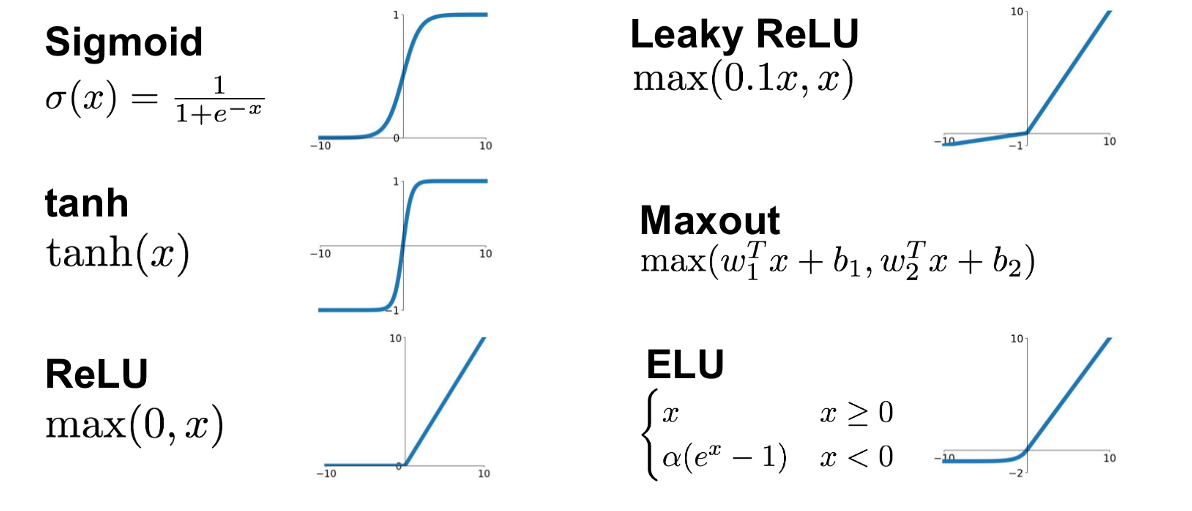
\includegraphics[width=1.\linewidth]{Chapters/items/chap2_6.jpg}
        \end{center}
        \label{fig: chap2_6}
    \end{subfigure}
    \caption{Một số hàm kích hoạt thường được sử dụng}
\end{figure}

\newpage
\subsection{Lớp gộp}

Sau hàm kích hoạt, thông thường chúng ta sử dụng lớp gộp. Một số loại lớp gộp phổ biến như là max-pooling, average pooling,
với chức năng chính là giảm chiều của tầng trước đó. Với một lớp gộp có kích thước 2x2,
các bạn cần phải trượt bộ lọc 2x2 này trên những vùng ảnh có kích thước tương tự rồi sau đó tính giá trị lớn nhất,
hay trung bình cho vùng ảnh đó.

\begin{figure}
    \begin{subfigure}{1.\textwidth}
        \begin{center}
            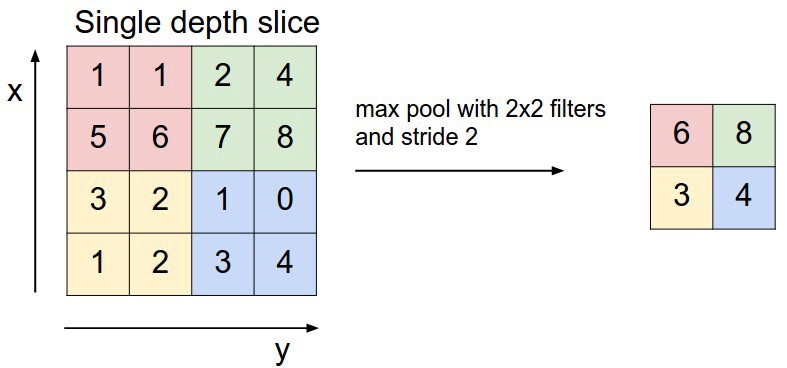
\includegraphics[width=1.\linewidth]{Chapters/items/chap2_7.jpg}
        \end{center}
        \label{fig: chap2_7}
    \end{subfigure}
    \caption{Ví dụ về max-pooling}
\end{figure}

Ý tưởng đằng sau lớp gộp là vị trí tuyết đối của những đặc trưng trong không gian ảnh không
còn cần cần thiết, thay vào đó vị trí tương đối giữ các đặc trưng đã đủ để phân loại đối tượng.
Hơn giảm tầng pooling có khả năng giảm chiều cực kì nhiều, làm hạn chế overfit,
và giảm thời gian huấn luyện tốt.

\subsection{Lớp kết nối đầy đủ}

Lớp cuối cùng của mô hình CNN trong bài toán phân loại ảnh là lớp kết nối đầy đủ.
Lớp này có chức năng chuyển ma trận đặc trưng ở tầng trước thành các vector chứa xác suất của các
đối tượng cần được dự đoán.

Quá trình huấn luyện mô hình CNN cho bài toán phân loại ảnh cũng tương tự như huấn luyện các
mô hình khác. Cần có hàm đánh giá mất mát để tính sai số giữa dự đoán của mô hình và nhãn chính xác,
để sử dụng cơ chế của thuật toán lan truyền ngược (backprobagation) cho quá trình cập nhật trọng số.

\begin{figure}
    \begin{subfigure}{1.\textwidth}
        \begin{center}
            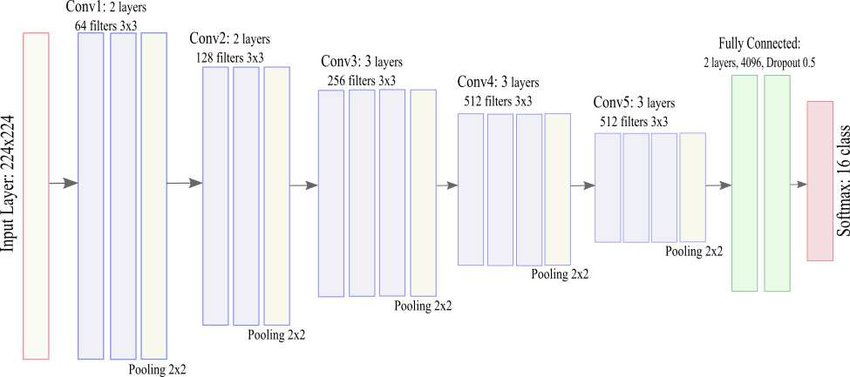
\includegraphics[width=1.\linewidth]{Chapters/items/chap2_8.jpg}
        \end{center}
        \label{fig: chap2_8}
    \end{subfigure}
    \caption{Một CNN đơn giản với đầy đủ các lớp}
\end{figure}

\newpage
\section{Máy dò khuôn mặt (Face detector)}

Để xác định các khuôn mặt\cite{detectface} trong các ảnh chứa nhiều yếu tố ngoại cảnh, và trích xuất các khuôn mặt đưa vào các
mô hình học sâu tiến hành trích xuất các đặc trưng của các khuôn mặt này thì phải dùng các máy dò khuôn mặt.

Hiện này có rất nhiều các máy dò khuôn mặt\cite{detectface1} được thiết kế bằng các mô hình học sâu khác nhau, ngay cả những máy dò được
thiết kế bằng các thuật toán xử lý ảnh thông thường cũng đã được phát triển và đạt hiệu quả tốt.
Ví dụ như các máy dò được tích hợp trong OpenCV (máy dò 5 điểm, 9 điểm, 68 điểm trên khuôn mặt). Nhưng để đạt được hiệu quả
tốt nhất có thể thì tôi sử dụng 1 máy dò có tên MTCNN (Multi-task Cascaded Convolutional Networks) được sử dụng phố biến
trong các hệ thống đòi hỏi sự chính xác cao.

\begin{figure}
    \begin{subfigure}{1.\textwidth}
        \begin{center}
            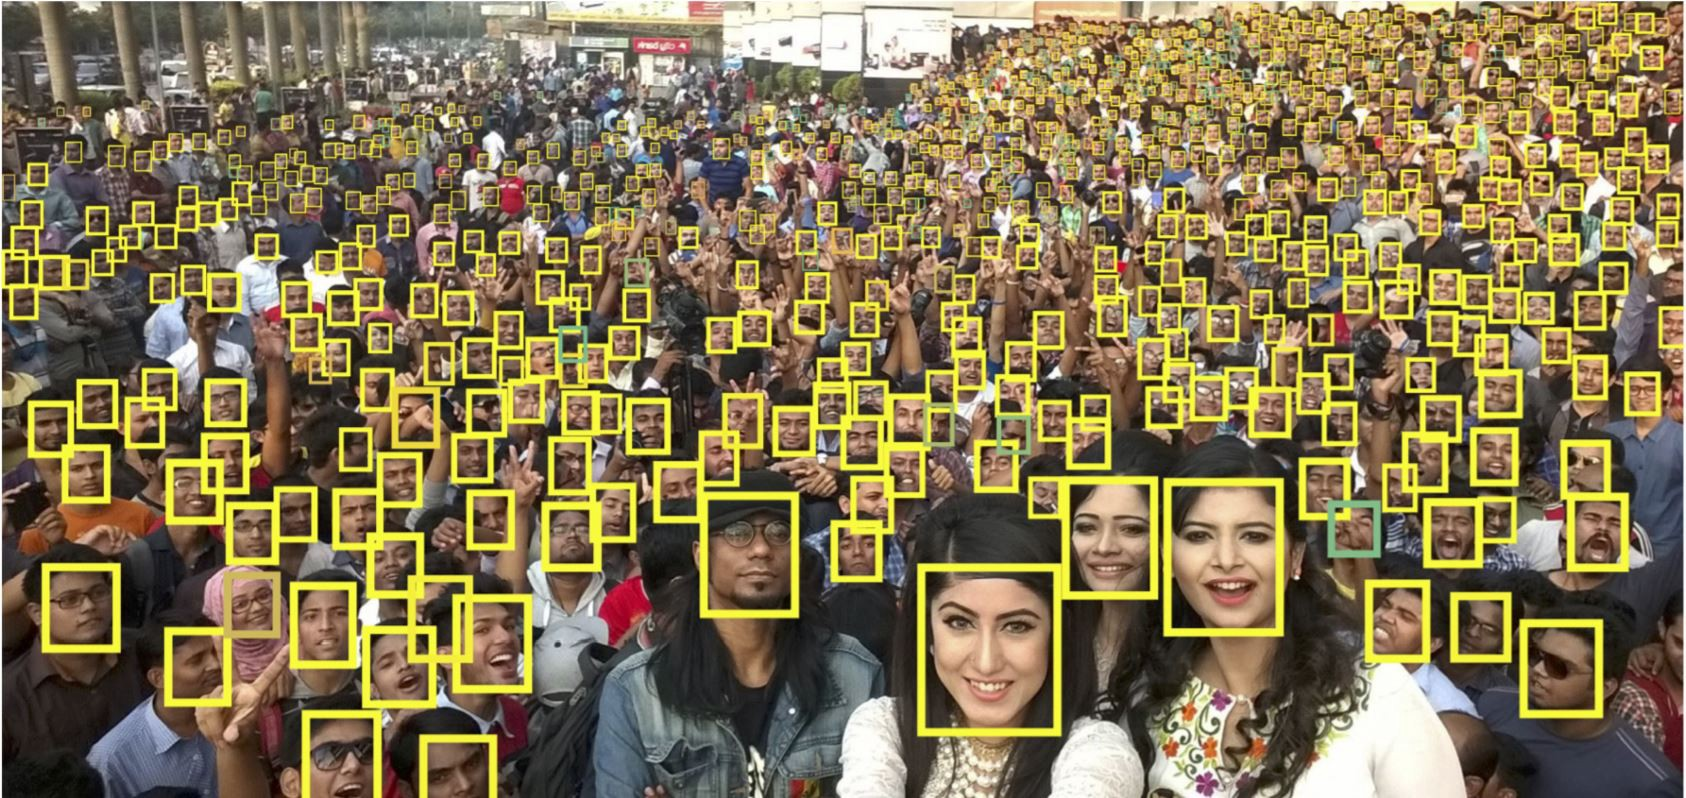
\includegraphics[width=1.\linewidth]{Chapters/items/chap2_test.jpg}
        \end{center}
        \label{fig: chap2_test}
    \end{subfigure}
    \caption{Ví dụ máy dò khuôn mặt}
\end{figure}

\newpage
\subsection{MTCNN}

MTCNN\cite{mtcnn} là viết tắt của Multi-task Cascaded Convolutional Networks (Mạng đa năng xếp tầng đa tác vụ).
Nó là bao gồm 3 mạng CNN xếp chồng và đồng thời hoạt động khi detect khuôn mặt.
Mỗi mạng có cấu trúc khác nhau và đảm nhiệm vai trò khác nhau trong task.
Đầu ra của MTCNN là vị trí khuôn mặt và 5 điểm trên mặt: mắt, mũi, miệng…

MTCNN hoạt động theo 3 bước, mỗi bước có một mạng neural riêng lần lượt là: P-Net, R-Net và O-net

\begin{figure}
    \begin{subfigure}{1.\textwidth}
        \begin{center}
            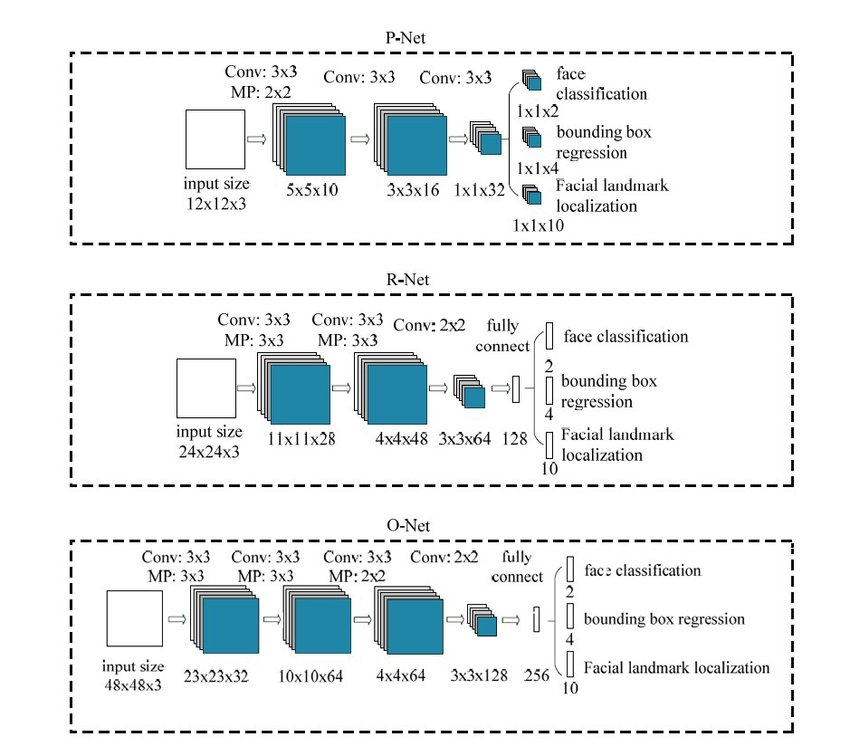
\includegraphics[width=1.\linewidth]{Chapters/items/chap2_9.jpg}
        \end{center}
        \label{fig: chap2_9}
    \end{subfigure}
    \caption{Các mạng neural trong MTCNN}
\end{figure}

\newpage
Với mỗi bức ảnh đầu vào, nó sẽ tạo ra nhiều bản sao của hình ảnh đó với các kích thước khác nhau.

Tại P-Net, thuật toán sử dụng 1 kernel 12x12 chạy qua mỗi bức hình để tìm kiếm khuôn mặt.

\begin{figure}
    \begin{subfigure}{1.\textwidth}
        \begin{center}
            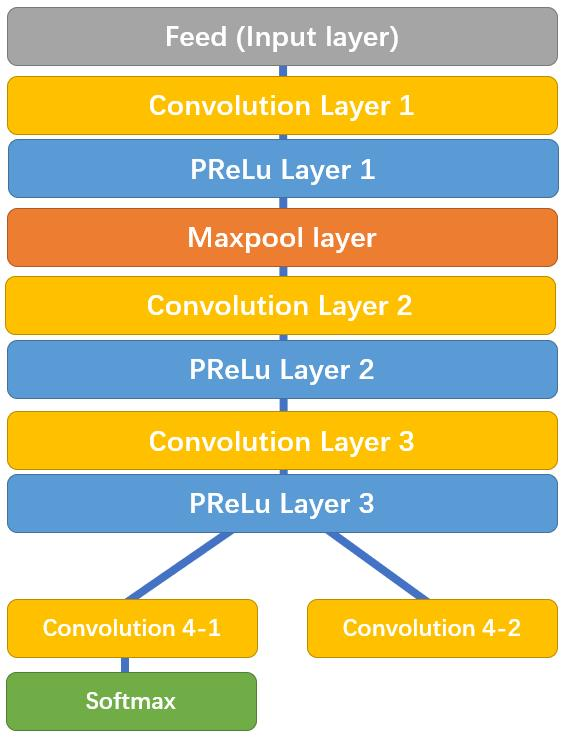
\includegraphics[width=0.6\linewidth]{Chapters/items/chap2_10.jpg}
        \end{center}
        \label{fig: chap2_10}
    \end{subfigure}
    \caption{Mô hình P-Net}
\end{figure}

\newpage
Sau lớp convolution thứ 3, mạng chia thành 2 lớp. Convolution 4-1 đưa ra xác suất của một khuôn mặt
nằm trong mỗi bounding boxes, và Convolution 4-2 cung cấp tọa độ của các bounding boxes.

R-Net có cấu trúc tương tự vói P-Net. Tuy nhiên sử dụng nhiều layer hơn.
Tại đây, network sẽ sử dụng các bounding boxes được cung cấp từ P-Net và tinh chỉnh là tọa độ.

\begin{figure}
    \begin{subfigure}{1.\textwidth}
        \begin{center}
            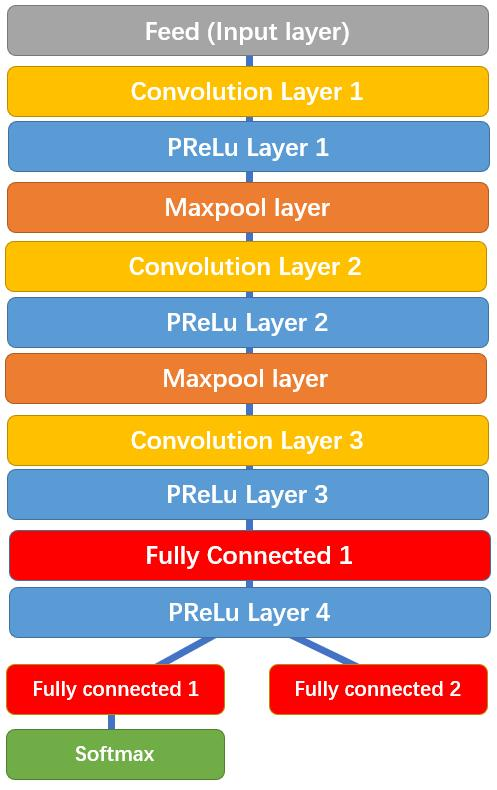
\includegraphics[width=0.6\linewidth]{Chapters/items/chap2_11.jpg}
        \end{center}
        \label{fig: chap2_11}
    \end{subfigure}
    \caption{Mô hình R-Net}
\end{figure}

\newpage
Tương tự R-Net chia ra làm 2 layers ở bước cuối, cung cấp 2 đầu ra đó là tọa độ
mới của các bounding boxes, cùng độ tin tưởng của nó.

O-Net lấy các bounding boxes từ R-Net làm đầu vào và đánh dấu các tọa độ của các mốc trên khuôn mặt.

\begin{figure}
    \begin{subfigure}{1.\textwidth}
        \begin{center}
            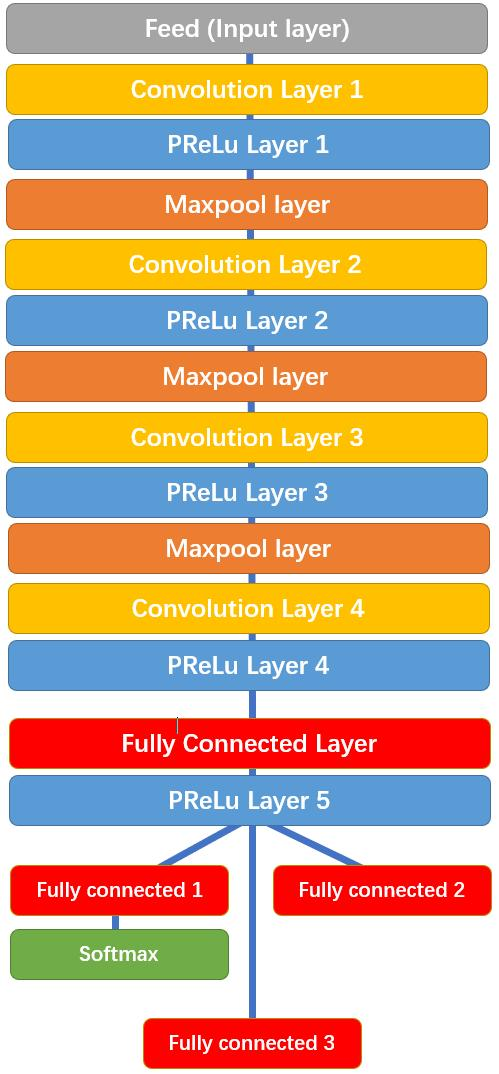
\includegraphics[width=0.55\linewidth]{Chapters/items/chap2_12.jpg}
        \end{center}
        \label{fig: chap2_12}
    \end{subfigure}
    \caption{Mô hình O-Net}
\end{figure}


Ở bước này, thuật toán đưa ra 3 kết quả đầu ra khác nhau bao gồm: 
xác suất của khuôn mặt nằm trong bounding box, tọa độ của bounding box và
tọa độ của các mốc trên khuôn mặt (vị trí mắt, mũi, miệng)

\begin{figure}
    \begin{subfigure}{1.\textwidth}
        \begin{center}
            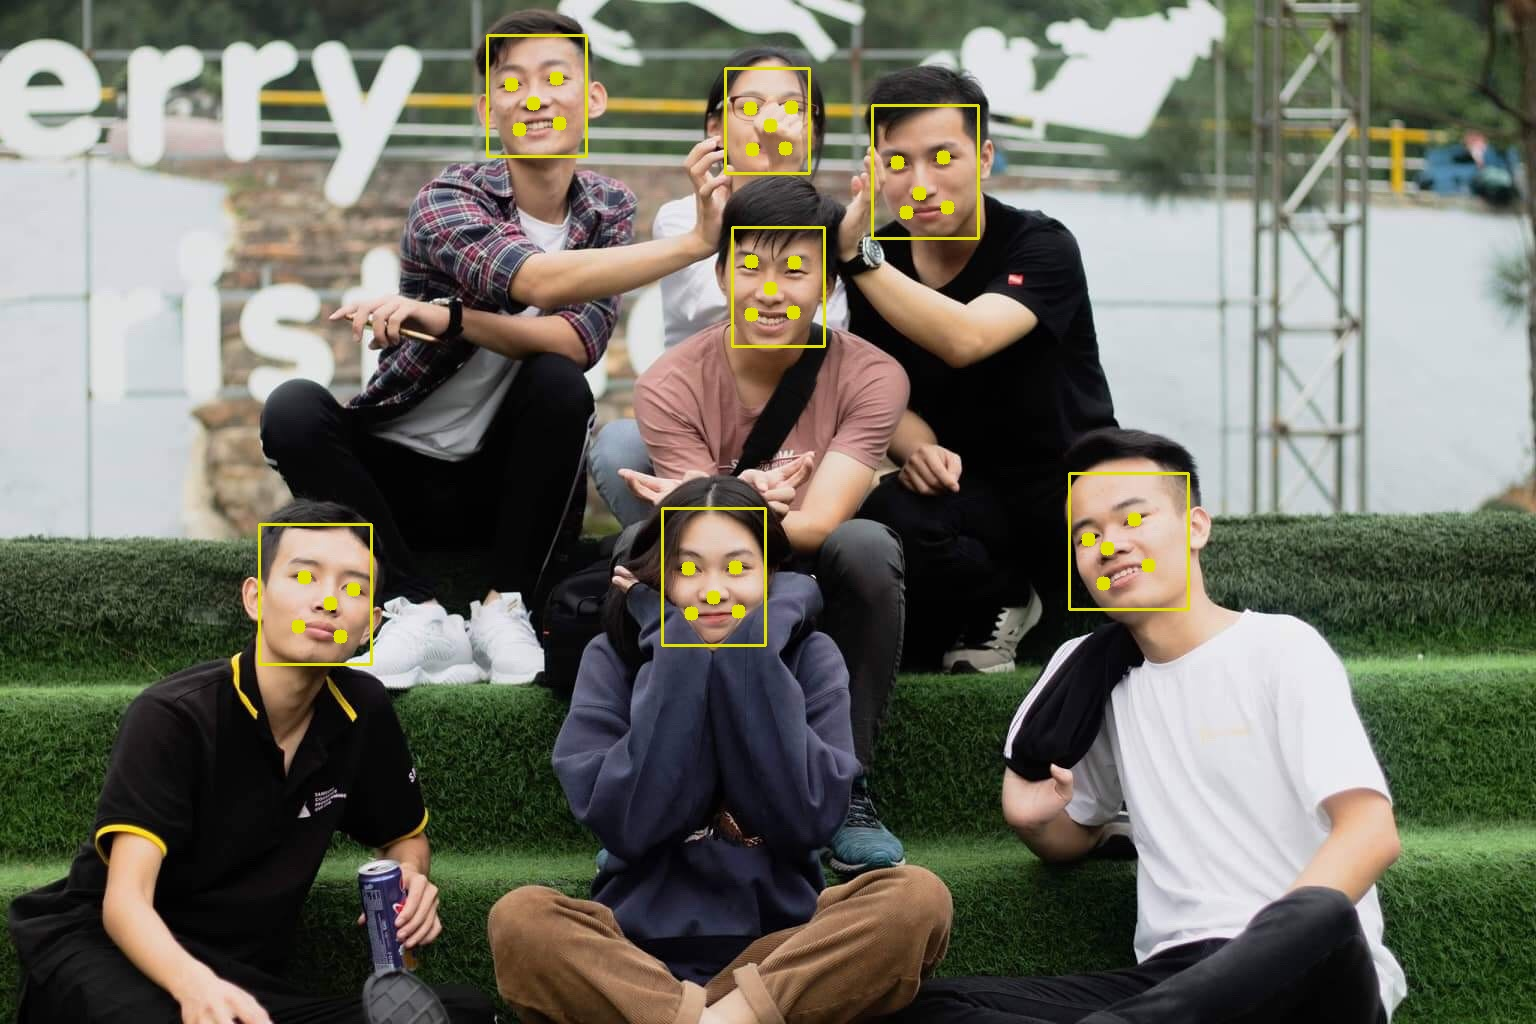
\includegraphics[width=1.\linewidth]{Chapters/items/chap2_14.jpg}
        \end{center}
        \label{fig: chap2_14}
    \end{subfigure}
    \caption{MTCNN xác định các khuôn mặt}
\end{figure}

\newpage
\section{Các kĩ thuật làm giàu dữ liệu (Data agumentation)}

Hiện nay các kĩ thuật làm giàu dữ liệu\cite{Augmentation} đang ngày các phát triển và phổ biến, khiến cho dữ liệu tăng lên
mạnh mẽ mà vẫn dữ được tính đặc trưng

Các kĩ thuật thường được sử dụng phổ biến là: Lật, xoay, phóng to, thu nhỏ, gây nhiễu, cắt, ...

Ngoài ra còn có các kĩ thuật nâng cao khác như là: sử dụng phép nội suy, GAN, đối xứng, bọc, ...

Còn rất nhiều những kĩ thuật phức tạp khác nhau và học sâu lại được sử dụng để giải quyết vấn đề này


\begin{figure}
    \begin{subfigure}{1.\textwidth}
        \begin{center}
            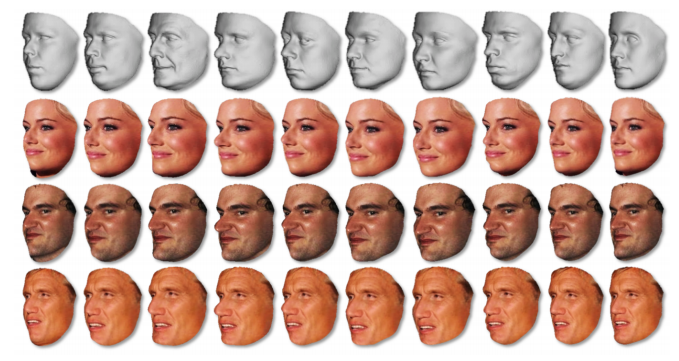
\includegraphics[width=1.\linewidth]{Chapters/items/chap3_6.jpg}
        \end{center}
        \label{fig: chap3_6}
    \end{subfigure}
    \caption{Làm giàu dữ liệu 3D sử dụng học sâu}
\end{figure}


\newpage
\section{Các thuật toán học sâu sử dụng trong nhận diện khuôn mặt}
\subsection{One-shot learning}

One-shot learning là thuật toán học có giám sát mà mỗi một người chỉ cần 1 vài,
rất ít hoặc thậm chí chỉ 1 bức ảnh duy nhất (để khỏi tạo ra nhiều biến thể).
Từ đầu vào là bức ảnh của một người, chúng ta sử dụng một kiến trúc CNN
đơn giản để dự báo người đó là ai.
Tuy nhiên nhược điểm của phương pháp này là chúng ta phải huấn luyện lại thuật
toán thường xuyên khi xuất hiện thêm một người mới vì số lượng của đầu ra thay đổi tăng lên 1.
Rõ ràng là không tốt đối với các hệ thống nhận diện khuôn mặt của một công ty vì số lượng người luôn biến động theo thời gian.

\subsection{Learning similarity}

Phương pháp này dựa trên một phép đo khoảng cách giữa 2 bức ảnh, thông thường là các định
mức chuẩn L1 hoặc L2 sao cho nếu 2 bức ảnh thuộc cùng một người thì khoảng cách là
nhỏ nhất và nếu không thuộc thì khoảng cách sẽ lớn hơn.

\begin{figure}
    \begin{subfigure}{1.\textwidth}
        \begin{center}
            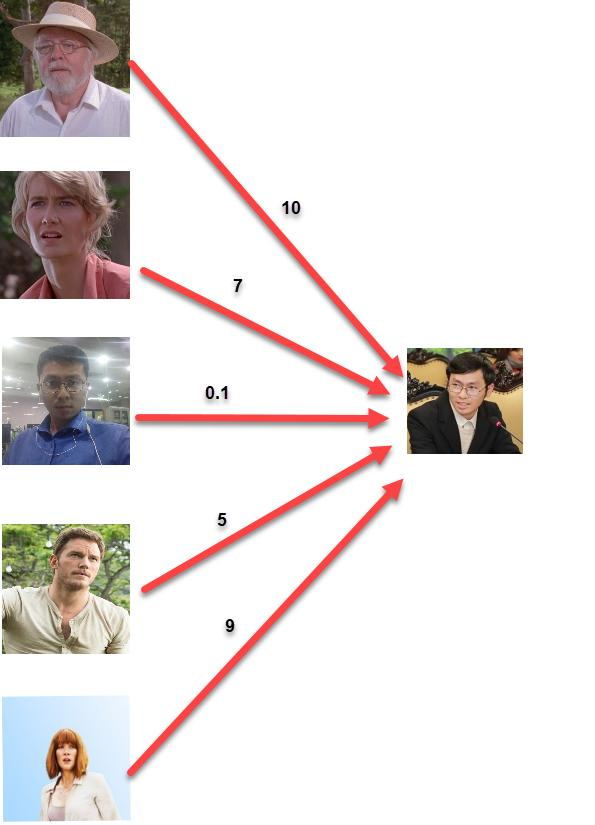
\includegraphics[width=0.5\linewidth]{Chapters/items/chap2_15.jpg}
        \end{center}
        \label{fig: chap2_15}
    \end{subfigure}
    \caption{Learning similarity}
\end{figure}

Learning similarity có thể trả ra nhiều hơn một ảnh là cùng loại với ảnh đầu vào tùy theo ngưỡng threshold.

Ngoài ra phương pháp này không bị phụ thuộc vào số lượng classes.
Do đó không cần phải huấn luyện lại khi xuất hiện class mới.
Điểm mấu chốt là cần xây dựng được một model encoding đủ tốt để chiếu các bức
ảnh lên một không gian eucledean n chiều. Sau đó sử dụng khoảng cách để quyết
định nhãn của chúng.

Như vậy learning similarity có ưu điểm hơn so với one-shot learning khi không phải
huấn luyện lại model khi mà vẫn tìm ra được ảnh tương đồng.
Vậy làm thế nào để học được biểu diễn của ảnh trong không gian euledean n chiều?
Kiến trúc siam network sẽ giúp chúng ta thực hiện điều này một cách dễ dàng.

\subsection{Siam learning}

Những kiến trúc mạng mà khi bạn đưa vào 2 bức ảnh và mô hình sẽ trả lời chúng thuộc về
cùng 1 người hay không được gọi chung là Siam network.

Kiến trúc của Siam network dựa trên base network là một Convolutional neural network
đã được loại bỏ output layer có tác dụng encoding ảnh thành vector embedding.
Đầu vào của mạng siam network là 2 bức ảnh bất kì được lựa chọn ngẫu nhiên từ dữ liệu ảnh.
Output của Siam network là 2 vector tương ứng với biểu diễn của 2 ảnh input.
Sau đó đưa 2 vector vào hàm loss function để đo lường sự khác biệt giữa chúng.
Thông thường hàm loss function là một hàm chuẩn bậc 2.

\begin{figure}
    \begin{subfigure}{1.\textwidth}
        \begin{center}
            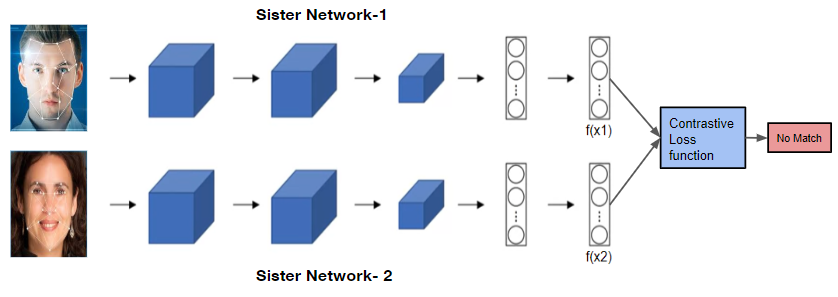
\includegraphics[width=1.\linewidth]{Chapters/items/chap2_16.jpg}
        \end{center}
        \label{fig: chap2_16}
    \end{subfigure}
    \caption{Siam learing}
\end{figure}

\newpage
Từ mô hình Convolutional neural network, mô hình trả ra 2 vector encoding là x1 và x2
biểu diễn cho lần lượt ảnh 1 và 2. x1 và x2 có cùng số chiều.
Hàm f(x) có tác dụng tương tự như một phép biến đổi qua layer fully connected
trong mạng neural network để tạo tính phi tuyến và giảm chiều dữ liệu về các kích thước nhỏ.
Thông thường là 128 đối đối với các mô hình pretrain.

\begin{figure}
    \begin{subfigure}{1.\textwidth}
        \begin{center}
            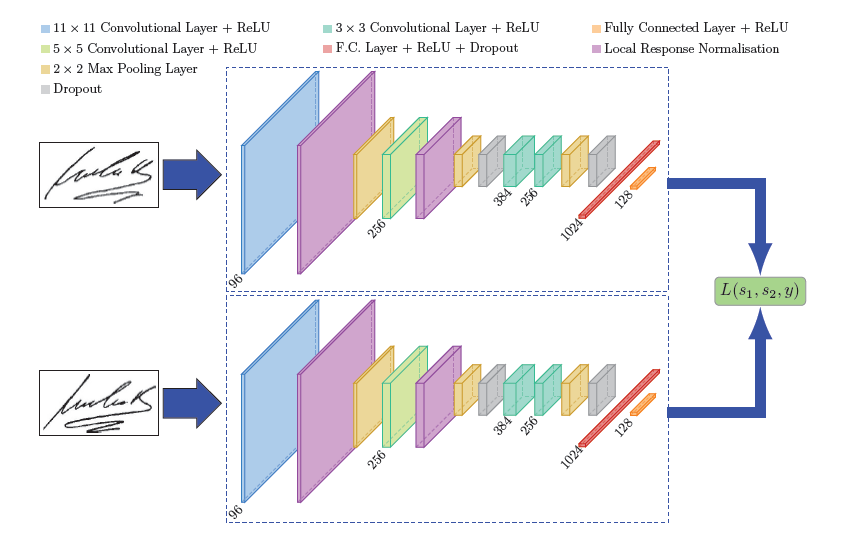
\includegraphics[width=1.\linewidth]{Chapters/items/siam.png}
        \end{center}
        \label{fig: siam}
    \end{subfigure}
    \caption{Siam network trong bài toán nhận dạng chữ ký}
\end{figure}


\newpage
\section{Mô hình học sâu được huấn luyện trước (Pre-train model)}
\subsection{Sử dụng mô hình được huấn luyện trước}

Mô hình huấn luyện trước là một mô hình được đào tạo bởi một người khác để giải quyết
một vấn đề tương tự. Thay vì xây dựng một mô hình từ đầu để giải quyết một vấn đề tương tự,
ta sử dụng mô hình được đào tạo về vấn đề khác làm điểm khởi đầu.
Thường thì những mô hình này là những mô hình rất lớn khó khăn trong việc huấn luyện
Một mô hình được đào tạo trước có thể không chính xác 100\%,
nhưng nó giúp tiết kiệm thời gian và công sức.

\subsection{Giới thiệu Facenet}

FaceNet\cite{FaceNet} là một mạng lưới thần kinh sâu được sử dụng để trích xuất các tính năng từ
hình ảnh của một mặt người. Nó được xuất bản vào năm 2015 bởi các nhà nghiên cứu của Google.

\begin{figure}
    \begin{subfigure}{1.\textwidth}
        \begin{center}
            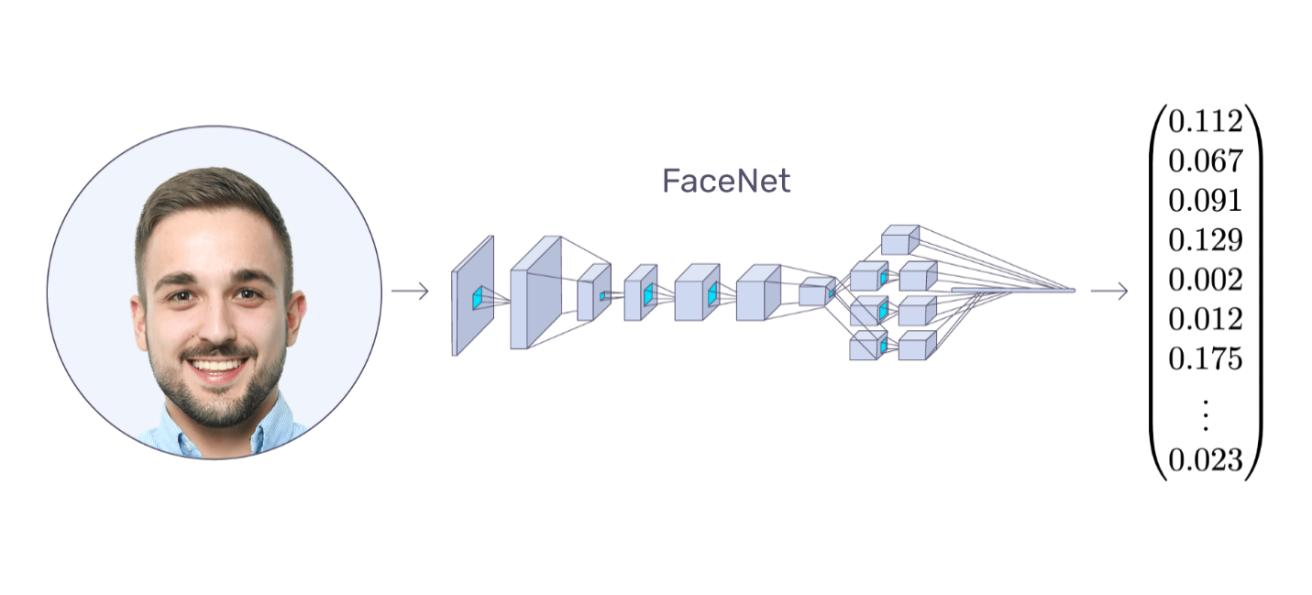
\includegraphics[width=1.\linewidth]{Chapters/items/chap2_17.jpg}
        \end{center}
        \label{fig: chap2_17}
    \end{subfigure}
    \caption{Facenet mã hóa hình ảnh khuôn mặt thành vector 128 chiều}
\end{figure}

FaceNet lấy hình ảnh của mặt người làm đầu vào và xuất ra một vector 128 chiều,
đại diện cho các tính năng quan trọng nhất của khuôn mặt.
Trong học máy, vector này được gọi là nhúng (embeddings).
Tại sao phải nhúng? Bởi vì tất cả các thông tin quan trọng từ một hình ảnh được nhúng
vào vector này. Về cơ bản, FaceNet lấy một mặt người và nén nó thành một vector gồm 128 số.
Khuôn mặt cần định danh cũng có nhúng tương tự.

Facenet chính là một dạng siam network có tác dụng biểu diễn các bức ảnh trong một không
gian eucledean n chiều (thường là 128) sao cho khoảng cách giữa các vector nhúng(embedding)
càng nhỏ, mức độ tương đồng giữa chúng càng lớn.

Hầu hết các thuật toán nhận diện khuôn mặt trước facenet đều tìm cách biểu diễn
khuôn mặt bằng một vector nhúng (embedding) thông qua một layer bottle neck có tác dụng
giảm chiều dữ liệu: 

\begin{itemize}
    \item Tuy nhiên hạn chế của các thuật toán này đó là số lượng chiều embedding
          tương đối lớn (thường >= 1000) và ảnh hưởng tới tốc độ của thuật toán.
          Thường chúng ta phải áp dụng thêm thuật toán PCA để giảm chiều dữ liệu để giảm
          tốc độ tính toán.
    \item Hàm loss function chỉ đo lường khoảng cách giữa 2 bức ảnh.
          Như vậy trong một đầu vào huấn luyện chỉ học được một trong hai khả năng
          là sự giống nhau nếu chúng cùng 1 class hoặc sự khác nhau nếu chúng khác
          class mà không học được cùng lúc sự giống nhau và khác nhau trên cùng một
          lượt huấn luyện.
\end{itemize}

Facenet đã giải quyết cả 2 vấn đề trên bằng các hiệu chỉnh nhỏ nhưng mang lại hiệu quả lớn: 

\begin{itemize}
    \item Base network áp dụng một mạng convolutional neural network và giảm chiều dữ
          liệu xuống chỉ còn 128 chiều. Do đó quá trình suy diễn và dự báo nhanh hơn và
          đồng thời độ chính xác vẫn được đảm bảo.
    \item Sử dụng loss function là hàm triplet loss có khả năng học được đồng thời
          sự giống nhau giữa 2 bức ảnh cùng nhóm và phân biệt các bức ảnh không cùng nhóm.
          Do đó hiệu quả hơn rất nhiều so với các phương pháp trước đây.
\end{itemize}

\newpage
\subsection{Giới thiệu Mạng InceptionResnetV1}

Mạng InceptionResnetV1\cite{resnet} có là sự kết hợp giữa 2 mạng cơ sở là Inception Net hay còn gọi là GoogLe Net

Nó được giới thiệu năm 2016 bởi các kĩ sư của Google, và cho thấy hiệu quả mạnh mẽ trên những tập dữ liệu ảnh lớn
tiêu biểu là tập dữ liệu ImageNet.

\begin{figure}
    \begin{subfigure}{1.\textwidth}
        \begin{center}
            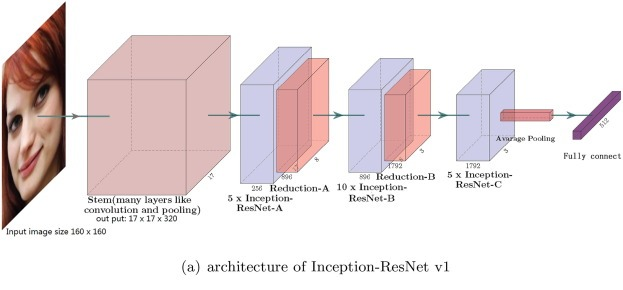
\includegraphics[width=1.\linewidth]{Chapters/items/chap2_19.jpg}
        \end{center}
        \label{fig: chap2_19}
    \end{subfigure}
    \caption{Cấu trúc tổng quan của InceptionResnetV1}
\end{figure}

InceptionResnetV1 là một mạng CNN kết hợp giữa các cấu trúc lớn với khoảng 23 triệu tham số trong mạng đồng nghĩa với
mỗi khi cho ảnh đi qua mạng này phải thức hiện 23 triệu phép tính, còn chưa kể trong quá trình huẩn luyện
mạng này phải thực hiện rất nhiều phép tính để thay đổi các tham số.

Chính vì sự khổng lồ của nó nên đã gây ra sự khó khăn trong quá trình huấn luyện, với những điều kiện như: 
lượng dữ liệu cho huấn luyện phải thật sự lớn (lên tới hàng chục triệu ảnh với hàng triệu khuôn mặt),
phần cứng hỗ trợ tính toán tốn kém, tài nguyên lưu trữ lớn, ...

Rất may mắn rằng có các tổ chức với lợi thế về dữ liệu, tài nguyên phần cứng đã huấn luyện thành công
các mạng này với những kết quả có độ chính xác cực cao.

Nên tôi đã sử dụng InceptionResnetV1 làm mạng cơ sở cho hệ thống này

\newpage
\subsection{Kĩ thuật đánh giá bộ ba (Triplet loss)}
Trong facenet, quá trình mã hóa của CNN đã giúp ta mã hóa bức ảnh về 128 chiều.
Sau đó những vector này sẽ làm đầu vào cho hàm đánh giá bộ ba để đánh giá khoảng
cách giữa các vector.

\begin{figure}
    \begin{subfigure}{1.\textwidth}
        \begin{center}
            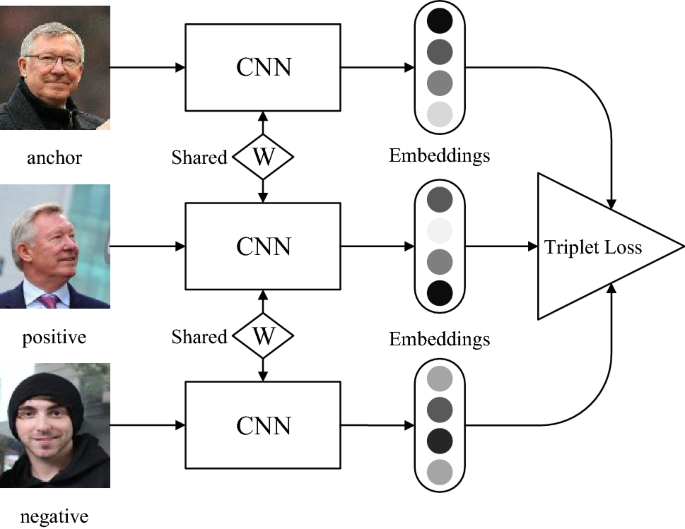
\includegraphics[width=1.\linewidth]{Chapters/items/chap2_18.jpg}
        \end{center}
        \label{fig: chap2_18}
    \end{subfigure}
    \caption{Mô hình sử dụng hàm đánh giá bộ ba}
\end{figure}

Mục tiêu của triplet loss là đảm bảo rằng: 
\begin{itemize}
    \item Hai ví dụ có cùng nhãn có các phần nhúng của chúng gần nhau trong không gian nhúng.
    \item Hai ví dụ với các nhãn khác nhau có các nhúng của chúng ở xa nhau.
\end{itemize}

Để áp dụng triple loss, chúng ta cần lấy ra 3 bức ảnh trong đó có một bức ảnh là anchor.
Trong 3 ảnh thì ảnh anchor được cố định trước.
Chúng ta sẽ lựa chọn 2 ảnh còn lại sao cho một ảnh là negative
(của một người khác với anchor) và một ảnh là positive (cùng một người với anchor).

Công thức --------------------------------------------------------------------

Mục tiêu của hàm triplet loss là tối thiểu hóa khoảng cách giữa 2 ảnh khi chúng là
negative và tối đa hóa khoảng cách khi chúng là positive.
Như vậy chúng ta cần lựa chọn các bộ 3 ảnh sao cho: 
\begin{itemize}
    \item Ảnh Anchor và Positive khác nhau nhất: cần lựa chọn để khoảng cách d(A,P) lớn.
          Điều này cũng tương tự như bạn lựa chọn một ảnh của mình hồi nhỏ so với hiện tại để
          thuật toán học khó hơn. Nhưng nếu nhận biết được thì nó sẽ thông minh hơn.
    \item Ảnh Anchor và Negative giống nhau nhất: cần lựa chọn để khoảng cách d(A,N)
          d(A,N) nhỏ. Điều này tương tự như việc thuật toán phân biệt được ảnh của một người
          anh em giống bạn.
\end{itemize}

\begin{figure}
    \begin{subfigure}{0.8\textwidth}
        \begin{center}
            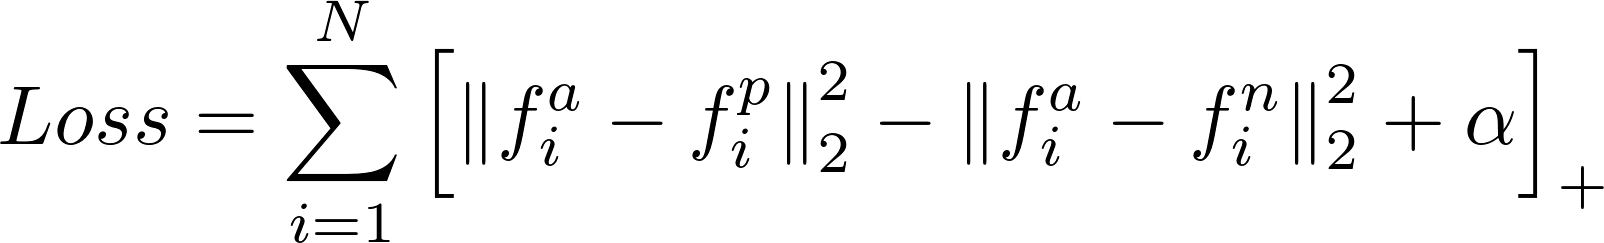
\includegraphics[width=1.\linewidth]{Chapters/items/fomura.png}
        \end{center}
        \label{fig: fomura}
    \end{subfigure}
    \caption{Công thức của hàm đánh giá bộ ba}
\end{figure}


